\documentclass[12pt,letterpaper]{article}
\usepackage[utf8]{inputenc}
\usepackage{times}
\usepackage{authblk}
\usepackage{graphicx}
\usepackage{placeins}

\title{StudyUp - USSA}

\author[1]{Yukon Vinecki}
\author[2]{Chandler Petersen}
\author[3]{Calvin Todorovich}
\author[4]{Moyez Ikhlas}
\affil[1]{vineckiy, EECS - Oregon State University}
\affil[2]{petercha, EECS - Oregon State University}
\affil[3]{todorovc, EECS - Oregon State University}
\affil[4]{ikhlasm, EECS - Oregon State University}

\usepackage[parfill]{parskip}
\begin{document}

\pagenumbering{roman}
\maketitle
\clearpage
\tableofcontents
\clearpage
\pagenumbering{arabic}

\section{User Stories and Corresponding Tasks}
\textbf{Bold} items are due this week. Plain text are due next week. \textit{Italic} items are nice-to-haves. Tasks are in order of which should be completed first to last. At the end of each task, there is a time estimate in parentheses indicating how long it would take a pair of programmers, working together, to complete the task.
\begin{enumerate}
\item \textbf{Ability to create a study group.}
	\begin{enumerate}
	\item Implement a "Create Group" form for the user to fill out.(1 day)
    \item Make a "Create" button on the "Create Group" form. (1 hour)
    \item Store new group's information in the database. (1 day)
    \item Navigate to the "View" UI after group is created.(1 hour)
	\end{enumerate}
\item \textit{Search for a class-oriented study group.}
	\begin{enumerate}
	\item Save all active group data in the database. (3 hours)
    \item Implement a search bar to query the database. (1 hour)
    \item Return all matches from the database that match with query. (1 hour)
	\end{enumerate}
\item Cancel a study group.
	\begin{enumerate}
	\item Create a "Cancel" button on the "View" UI. (1 hour)
    \item Create functionality to check what kind of user it is (i.e. study group administrator or user who has joined a group.) Make sure that only a study group administrator is presented with the "cancel" option when looking at the "View" UI. (2 days)
    
	\end{enumerate}
\item Website is easy to navigate.
	\begin{enumerate}
	\item Create navigation bar at top of page with links to navigate to all possible UI pages present.(1 hour)
    \item Ensure link names are logical regarding where they will navigate to, as well as making sure they are placed in such a way that is intuitive for the user. (half hour)
	\end{enumerate}
\item \textbf{Login with canvas login.}
	\begin{enumerate}
	\item Research Canvas API standard and calls that will be used.(1 week)
    \item Implement validating user token on site. (3 hours)
    \item Add standard user authentication to website. (2 hours)
    \item Integrate canvas login into authentication framework. (2 hour)
	\end{enumerate}
\item \textbf{Join group easily.}
	\begin{enumerate}
	\item Design UI element(s) to solve request.(1 day)
    \item Implement designed UI on website page. (1 day)
    \item Make elements functionality work. (1 week)
	\end{enumerate}
\item \textbf{See current study groups upon entering site.}
	\begin{enumerate}
	\item Pull active group information from the database. (2 hours)
    \item Design Home Page UI. (3 hours)
    \item Display information from the database on the Home Page. (1 hour)
	\end{enumerate}
\item \textit{Calendar of study groups.}
	\begin{enumerate}
	\item Integrate with the Canvas API. (3 days)
    \item Link newly created/joined groups with the Canvas calendar. (3 hours)
    \item Add the study groups as events on the calendar. (2 hours)
    \item Create a link on the navigation bar to the application's calendar. (half hour)
	\end{enumerate}
\item \textit{Campus map showing locations of study groups.}
	\begin{enumerate}
	\item Find an API for OSU's campus map. (2 hours)
    \item Do research on how to represent study groups on the map. (3 hours)
    \item Implement campus map integration. (4 days)
    \item Create link to the map in the application's navigation bar.(half hour)
	\end{enumerate}
\item \textit{Email notifications for events.}
	\begin{enumerate}
	\item Research automated email service. (1 day)
    \item Figure out how to use the service's API.(1 day)
    \item Create implementation for sending out email alerts if user joins, creates, leaves, or cancels a study group. (3 days)
	\end{enumerate}
\item \textit{Discussion board on study groups.}
	\begin{enumerate}
	\item Add data tables for messages in the database. (1 hour)
    \item determine what the UI for the discussion board will look like. (1 day)
    \item Add UI for the discussion board into the application. (2 days)
    \item Create a link to the discussion board on the application's navigation bar. (half hour)
	\end{enumerate}
\item Able to add class resources to group page. 
	\begin{enumerate}
	\item Create a text-box on "Create Study Group" form. (2 hours)
    \item Make sure entered information is saved to the database and updated on the "View" UI. (2 hours)
	\end{enumerate}
\item Access my canvas classes on the website.
	\begin{enumerate}
	\item Integrate with Canvas API. (3 days)
    \item Pull in user's classes into database and display on "Create Study Group" page. (3 days)
	\end{enumerate}
\item \textit{Access website from mobile device.}
	\begin{enumerate}
	\item Validate if application can be seen on a mobile device. Find out what works and what does not. (1 hour)
    \item Systematically address non-working aspects and adjust structure and functionality until it is mobile-compatible. (1 week)
	\end{enumerate}
\item Leave study group if accidentally join.
	\begin{enumerate}
	\item Create a new button "Leave", on the "View" UI. (1 hour)
    \item Finish database so that way users can be added and removed from groups. (3 days)
    \item Create functionality to check what kind of user it is (i.e. study group administrator or user who has joined a group.) (2 days)
    
	\end{enumerate}
\end{enumerate}

\clearpage
\section{UML Sequence Diagram/Spike}
\subsection{Canvas Login}
\begin{figure}[!htb]
  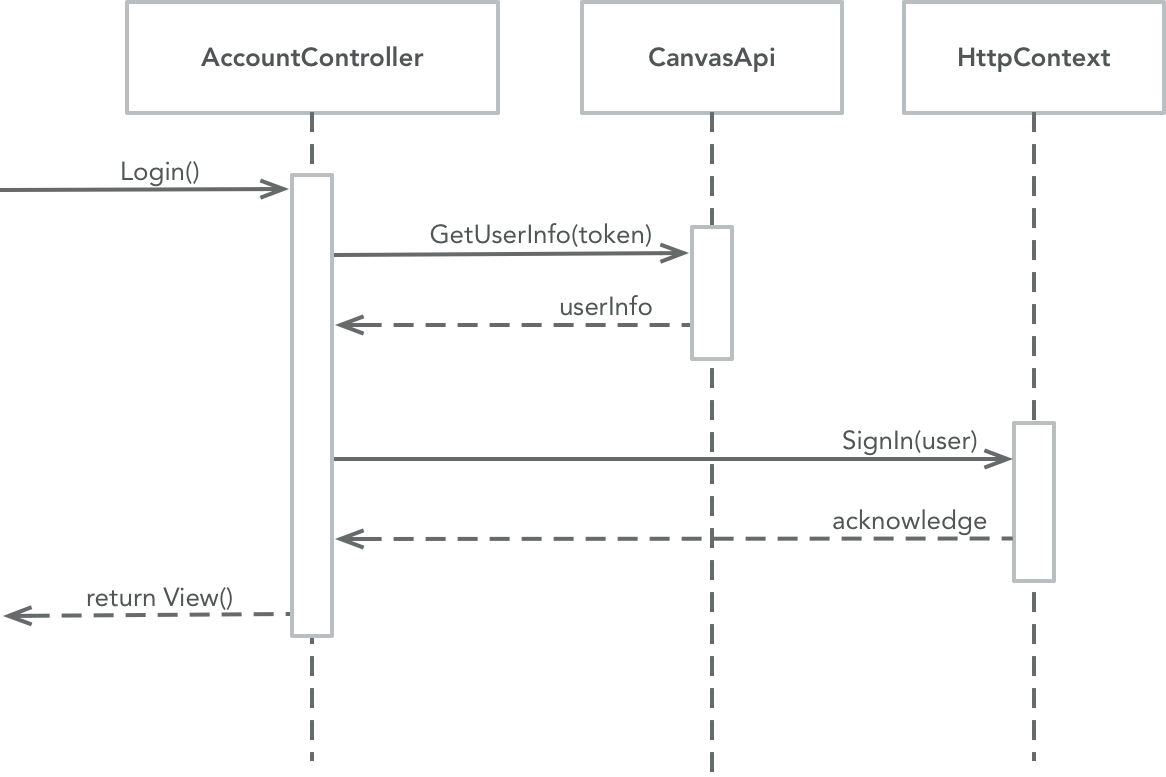
\includegraphics[width=\linewidth]{CanvasSigninUML.png}
  \caption{Canvas login sequence diagram.}
  \label{canvas_login}
\end{figure}
\clearpage

\subsection{Create study group}
\begin{figure}[!htb]
  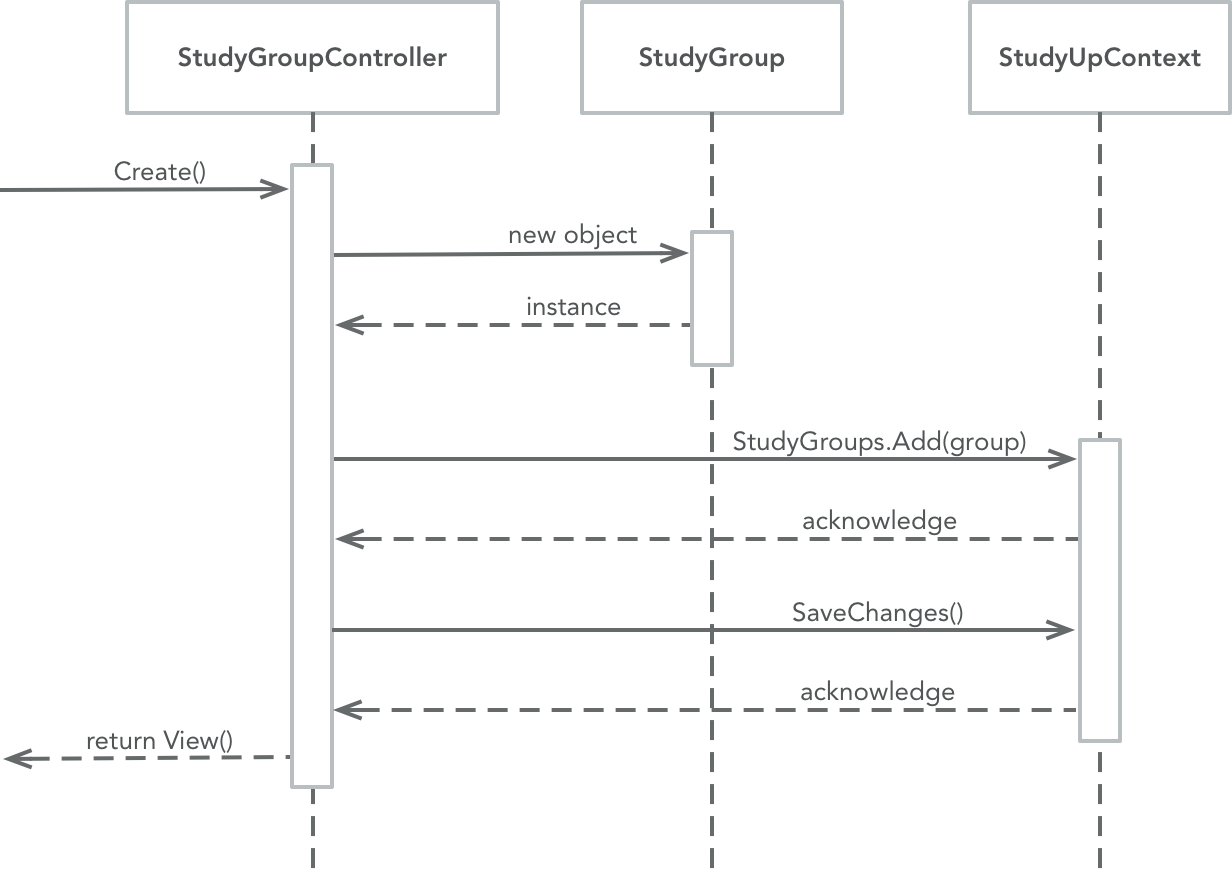
\includegraphics[width=\linewidth]{CreateGroupUML.png}
  \caption{Create group sequence diagram.}
  \label{create_group}
\end{figure}
\clearpage

\subsection{List current groups}
\begin{figure}[!htb]
  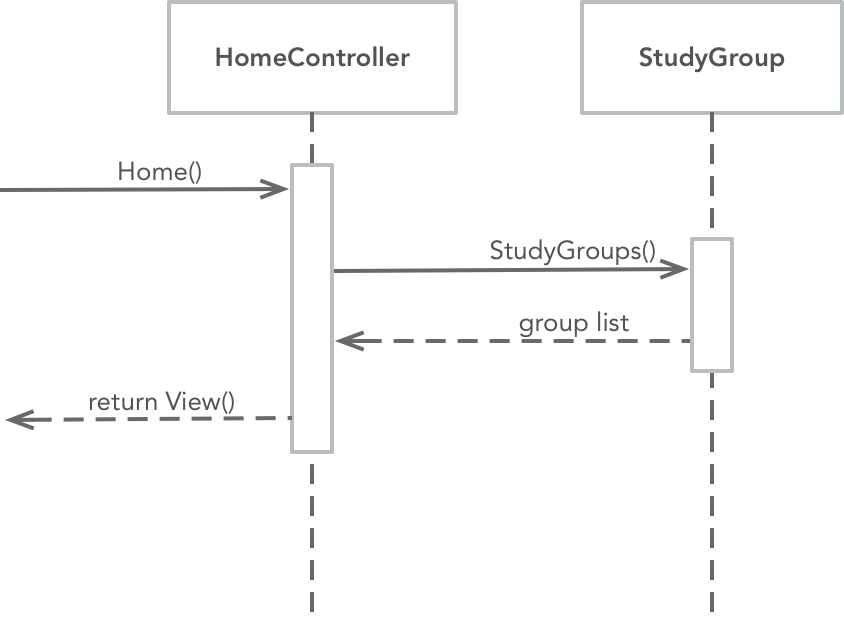
\includegraphics[width=\linewidth]{CurrentGroupsUML.png}
  \caption{List current groups sequence diagram.}
  \label{current_groups}
\end{figure}
\clearpage

\subsection{Join study group}
\begin{figure}[!htb]
  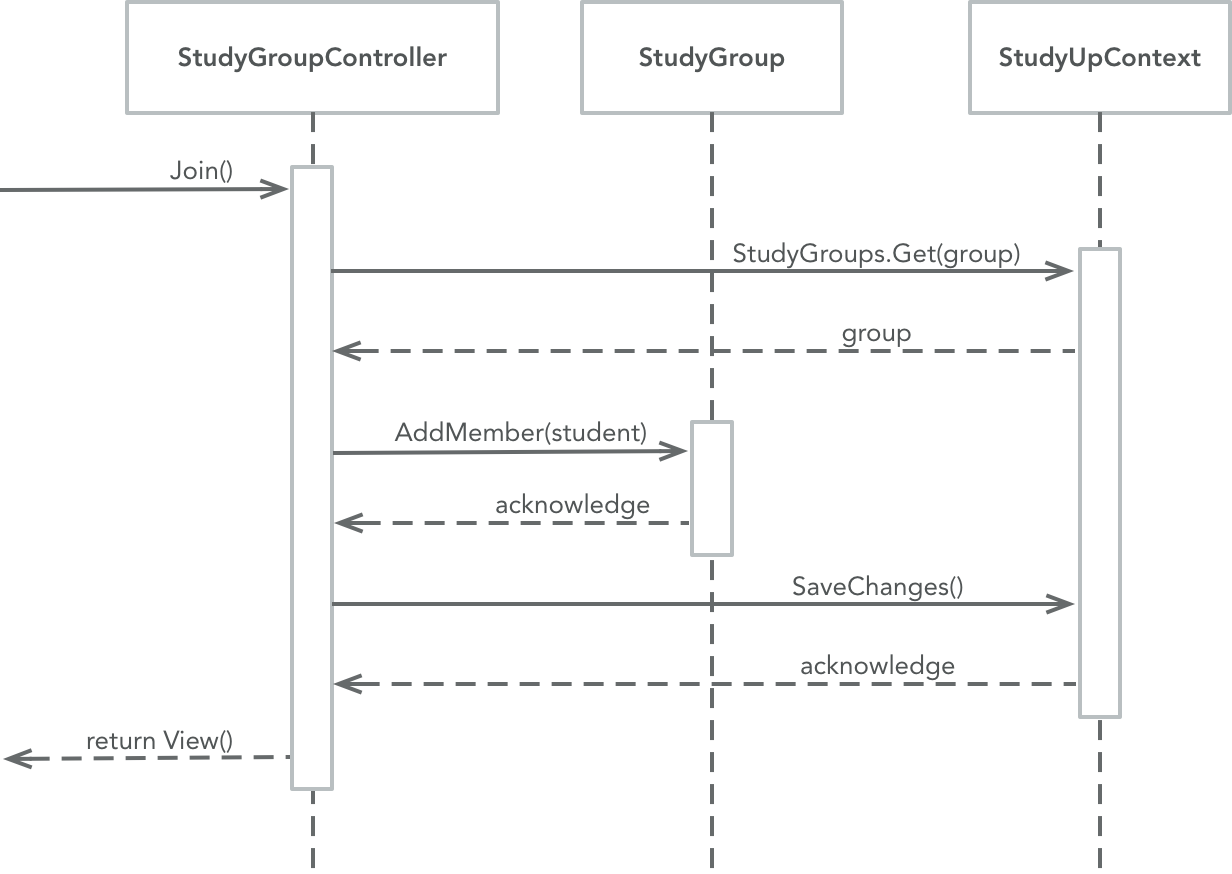
\includegraphics[width=\linewidth]{JoinGroupUML.png}
  \caption{Join study group sequence diagram.}
  \label{join_group}
\end{figure}
\clearpage

\section{The Stories Due Next Week}
\textbf{Ability to create a study group.}

Calvin is the developer who is assigned to this story. He has already started work developing the UI and is beginning work on the functionality. This work can be done in parallel with other stories.

\textbf{See current groups when entering site.}

Moyez is assigned to this story. He has designed the UI elements for the page and is now tasked with making it functional with real data. This functionality depends on canvas login to retrieve class data from page.

\textbf{Login with canvas login.}

Yukon is assigned to this story. This story has been implemented and validated to function properly. This item completed ahead of schedule allowing work on functionality for other stories to be properly tested.

\textbf{Join group easily.}

This story item is apart of viewing a study group which is assigned to Chandler. This involves having a visible button when viewing study groups to join the group. The UI element has already been implemented with the functionality to be completed next.

\clearpage
\section{Meeting Report}
This week the group met on Friday to check in on each group member's progress on implementing the functionality of their portion of the UI. Additionally, we discussed 15 user stories relevant to our application, as well as the corresponding tasks needed to meet the criteria of each user story.

Currently, the functionality the user login is complete. Otherwise, Yukon is working on the database so that way we can integrate in all parts of the UI and get a functioning application. Right now, however, we are all working with sample objects in effort to get each individual UI component functioning. Chandler is working "View", Calvin on "Create Study Group", and Moyez on "Find Study Group." Getting the database running and continuing to implement the functionality will be an ongoing goal for this week as well.

Chandler will work on the "View" functionality, Yukon will continue work on the database, Calvin will work on implementing the "Create Study Group" functionality, and Moyez will work on the "Find Study Group functionality." By next week, our goal is to have a rough functional version of the website.

We met with our customer and discussed the tasks. we found the proposed tasks reasonable and plan on implementing them. We are planning on meeting Tuesday and Friday in order to check in on each group member's progress and continue working on our implementations. 
\end{document}